\documentclass[a4paper,12pt]{article}

\usepackage{../latex/mystyle}
\addbibresource{ref.bib}

\begin{document}

\begin{center}
\begin{tabu} to \textwidth {lX[c]r}
    Groupe 1211 & \large{\textbf{Rapport~2}} & 14 octobre 2014 \\
    \hline
\end{tabu}
\end{center}

\section{Introduction}

Notre sujet d'étude étant la production d’ammoniac, en commençant par la synthèse de celui-ci à partir du reformage, il nous a été nécessaire de passer par l’étape de la gestion du plant. Ce rapport présente donc nos calculs et codes MATLAB du bilan de matière, en fonction de la température dans le réacteur et de la quantité d’ammoniac produite, du bilan d’énergie et finalement le calcul du nombre de tubes nécessaires à l’entrée des différents réactifs. 

\section{Flow-sheet rempli}

La figure~\ref{fig:flowsheet2} présente le flow-sheet que nous avons complété à l'aide des sources \cite{epa} et \cite{process-patent}.

\begin{figure}
    \centering
    \tikzstyle{reaction} = [
    rectangle, draw, thick, rounded corners, fill=black!10,
    text width=13em, text centered,
    minimum height=6em
]
\tikzstyle{inout} = [
    rectangle,
    node distance=6em,
    font=\footnotesize
]
\tikzstyle{ioside} = [
    inout,
    node distance=10em
]

\tikzstyle{thinflow} = [
    draw, -latex'
]
\tikzstyle{flow} = [
    thinflow, thick
]

\tikzstyle{flowing} = [
    text centered,
    font=\footnotesize,
    inner sep=.5em,
]

\begin{tikzpicture}[node distance=9em, auto]
    
    % Reaction boxes
    \node [reaction] (primary) {
        Reformage primaire \\[.3em]
        \footnotesize{
            (A) \ce{CH4 + H2O <-> CO + 3H2} \\
            (B) \ce{CO + H2O <-> CO2 + H2} \\
            (équilibre à la sortie)
        }
    };
    \node [reaction, below of=primary] (secondary) {
        Reformage secondaire \\[.3em]
        \footnotesize{
            (C) \ce{2CH4 + O2 -> 2CO + 4H2} \\
            (considérée complète)
        }
    };
    \node [reaction, below of=secondary] (shift) {
        Réacteurs Water-Gas-Shift \\[.3em]
        \footnotesize{
            (D) \ce{CO + H2O -> CO2 + H2} \\
            (considérée complète)
        }
    };
    \node [reaction, below of=shift] (sepa) {
        Séparation de \ce{CO2} et \ce{H2O} \\[.3em]
        \footnotesize{
            (considérée complète)
        }
    };
    \node [reaction, below of=sepa] (synthesis) {
        Synthèse de l'ammoniac et séparation \\
        \footnotesize{
            (E) \ce{N2 + 3H2 -> 2NH3} \\
            (considérée complète)
        }
    };
    \node [reaction, right of=primary, node distance=18em, fill=red!10] (oven)
    {
        Four \\[.3em]
        \footnotesize{
            \ce{CH4 + 2O2 -> CO2 + 2H2O} \\
            (complète)
        }
    };
    
    % Empty in-out boxes
    \node [inout, above of=primary] (in12) {\ce{CH4}, \ce{H2O}};
    \node [ioside, left of=secondary] (in3) {air};
    \node [ioside, right of=sepa, node distance=11em] (out12) {\ce{CO2}, \ce{H2O}};
    \node [ioside, right of=synthesis] (out3) {\ce{Ar}};
    \node [inout, below of=synthesis] (out4) {\ce{NH3}};
    \node [inout, above of=oven] (inoven) {\ce{CH4}, \ce{O2}};
    \node [inout, below of=oven] (outoven) {\ce{CO2}, \ce{H2O}};
    
    % In-out flows (thin arrows)
    \path [thinflow] (in12) -- (primary);
    \path [thinflow] (in3) -- (secondary);
    \path [thinflow] (sepa) -- (out12);
    \path [thinflow] (synthesis) -- (out3);
    \path [flow] (synthesis) -- (out4);
    \path [thinflow] (inoven) -- (oven);
    \path [thinflow] (oven) -- (outoven);

    % Energy flow
    \path [thinflow] (oven) --
    node [flowing, above] {chaleur}
    (primary);

    % Main flows
    \path [flow] (primary) --
    node [flowing, right]{
        \ce{CH4}, \ce{H2O}, \ce{CO}, \ce{CO2}, \ce{H2}
    }
    (secondary); 
    \path [flow] (secondary) --
    node [flowing, right]{
        \ce{H2O}, \ce{CO}, \ce{CO2}, \ce{H2}, \ce{N2}, \ce{Ar}
    }
    (shift);
    \path [flow] (shift) --
    node [flowing, right]{
        \ce{H2O}, \ce{CO2}, \ce{H2}, \ce{N2}, \ce{Ar}
    }
    (sepa);
    \path [flow] (sepa) --
    node [flowing, right]{
        \ce{H2}, \ce{N2}, \ce{Ar}
    }
    (synthesis);

\end{tikzpicture}

    \caption{Flow-sheet simplifiée du procédé de production d'ammoniac.}
    \label{fig:flowsheet2}
\end{figure}

\section{Bilan de matière}

Dans cette section nous allons utiliser ce que nous savons
sur les réactions pour trouver les différents débits de matière du procédé
en fonction du débit sortant de \ce{NH3}
et de la température du réformage primaire.

Il suffit \emph{a priori} de prendre ce débit
d’ammoniac désiré et remonter pas à pas
dans les différentes équations pour arriver aux réactifs de base
et ainsi savoir de combien de moles, ou de kilogrammes, de matière première
nous avons besoin.

Cependant, ce n’est pas si simple étant donné
que le procédé inclut des réactions à l’équilibre,
pour lesquelles certains réactifs ne réagissent pas complètement,
et accompagnent les produits dans les réactions suivantes.
De plus, certains réactifs sont ajoutés à différents endroits dans la chaine,
aux quantités inconnues, ce qui ajoute encore un niveau de complexité.

Nous avons donc cherché une solution plus générale et automatique.
Et cela signifie écrire un grand système d'équations et laisser notre environnement
de calcul numérique favori le résoudre (presque) tout seul.

\subsection{Inconnues et équations}

Commençons par déterminer nos inconnues et les relations dont nous disposons.

Pour les inconnues, nous choisissons les débits de moles suivants:
\begin{itemize}
    \item $\mathrm{in}_1$, $\mathrm{in}_2$, $\mathrm{in}_3$
        les entrées de \ce{CH4}, \ce{H2O} et air;
    \item $\mathrm{out}_1$, $\mathrm{out}_2$, $\mathrm{out}_3$,
        $\mathrm{out}_4$ les sorties de \ce{H2O}, \ce{CO2}, \ce{Ar} et \ce{NH3};
    \item $\alpha$, $\beta$, $\gamma$, $\delta$ et $\epsilon$
        les degrés d'avancement des cinq réactions.
\end{itemize}
Il s'agit bien de débits, que nous exprimerons en $\mole\per\second$,
car le procédé fonctionne en continu.%
\footnote{Toutefois, les calculs seraient identiques
pour un mode opératoire discret.}

En ce qui concerne les équations, nous pouvons exprimer:
\begin{itemize}
    \item la conservation de chacune des 9 espèces à travers le procédé:
        ce qui est apporté ou produit doit égaler ce qui est enlevé ce qui réagit;
    \item le débit de sortie de \ce{NH3}, imposé par l'utilisateur;
    \item les deux relations d'équilibre à la sortie du réacteur de réformage
        primaire.
\end{itemize}

Nous avons $3+4+5 = 12$ inconnues et $9+1+2 = 12$ équations,
donc le système est résolvable.

Les différentes inconnues et équations sont illustrées dans
la figure~\ref{fig:flows-matter}.
Les inconnues (entrées, sorties et réactions) sont représentées par des cercles,
tandis que les 9 relations de conservation de matière
sont représentées par des flèches entre les inconnues.

\begin{figure}
    \centering
    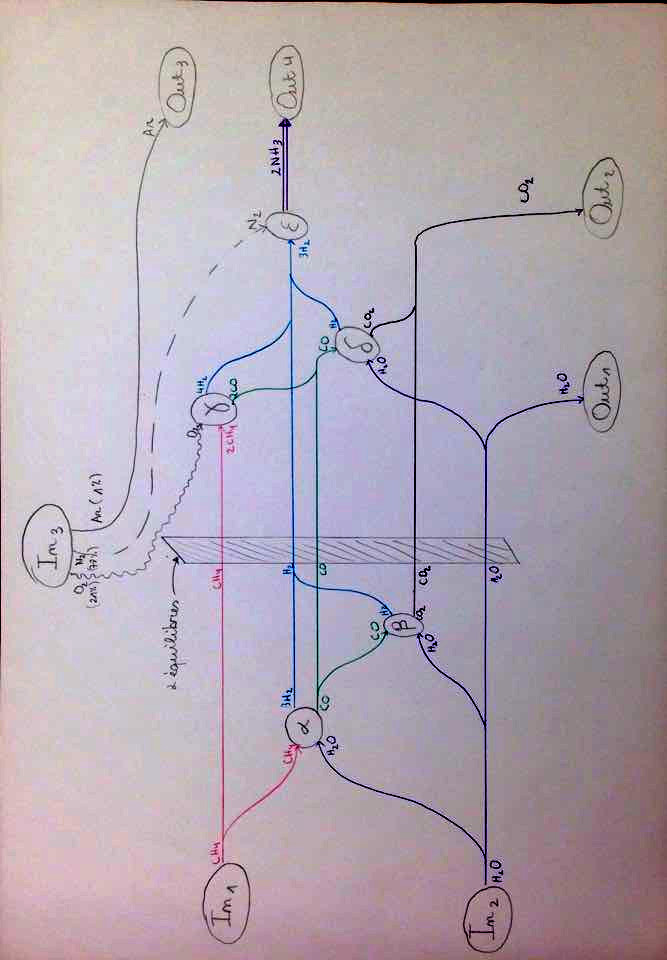
\includegraphics[width=\textwidth]{flows_matter}
    \caption{
        Procédé de production du point de vue de la matière.
        On remarque que les relations d'équilibres s'appliquent après que les deux
        réactions du reformage primaire aient eu lieu.
    }
    \label{fig:flows-matter}
\end{figure}

\subsection{Expression des équations}



\section{Bilan énergétique}
\section{Nombre de tubes}
\section{Outil de gestion}

\printbibliography[heading=bibintoc]

\end{document}
